\documentclass[a4paper,11pt]{article}
\usepackage[utf8]{inputenc}
\usepackage[T1]{fontenc}
\usepackage[french]{babel}
\usepackage{textcomp}
\usepackage{listings}
\usepackage{pdfpages}
\usepackage{array}

\title{PROJET\\ UE Méthodes de ranking et recommandations\\ 
		Sujet 5 : Simulation d'un Google Bombing}
\author{Maxime Gonthier - Laureline Martin}

\begin{document}

\pagenumbering{gobble}\clearpage
	\pagenumbering{gobble}\clearpage
	\maketitle
	\newpage\clearpage\pagenumbering{arabic}

\newpage
\tableofcontents
\newpage

On considère ici le graphe du web Stanford.txt. Ce graphe est modifié par l'ajout de sommets et d'arcs afin d'augmenter la valeur d'un sommet ciblé.\\
On considère que :\\
\begin{itemize}
	\item Les sommets représentent les pages du web.
	\item Les arcs représentent les liens dirigeant vers d'autres pages.
	\item Les valeurs des sommets représentent les pertinences calculés par l'algorithme pagerank.
	\item Le sommet cible représente la page dont on souhaite augmenter la pertinence.
\end{itemize}

\section{Tests initiaux et hypothèses}
	\subsection{Explication du code}
	\subsection{Résultats des tests initiaux}
		\subsubsection{Pagerank sur Stanford.txt (sans modification) :}
			281903 pages\\
			2312497 liens\\
			132 itérations\\
			27.627466 secondes\\
			\\
			On choisi d'attaquer ces différentes pages à pertinences différentes :\\
			Pertinence forte : Page 280545 - 9.96199e-05\\
			Pertinence moyenne : Page 281466 - 7.53954e-06\\
			Pertinence faible : Page 281574 - 6.05222e-07\\
			\\
		\subsubsection{Pagerank sur Stanford.txt (ajout de 10 sommets seuls) :}
			281913 pages\\
			2312507 liens\\
			132 itérations\\
			27.075775 secondes / 27.082188 secondes / 28.454464 secondes\\
			\\
			Cible à pertinence forte : 1.07873e-04\\
			Cible à pertinence moyenne : 1.26718e-05\\
			Cible à pertinence faible : 5.73756e-06\\
			\\
		\subsubsection{Pagerank sur Stanford.txt (ajout d'un anneau à 10 sommets) :}
			281913 pages\\
			2312508 liens\\
			132 itérations\\
			29.058716 secondes / 27.939356 secondes / 30.209354 secondes\\
			\\
			Cible à pertinence forte : 1.02068e-04\\
			Cible à pertinence moyenne : 9.06326e-06\\
			Cible à pertinence faible : 2.12916e-06\\
			\\
		\subsubsection{Pagerank sur Stanford.txt (ajout d'un graphe complet à 10 sommets) :}
			281913 pages\\
			2312588 liens\\
			132 itérations\\
			32.530811 secondes / 30.358072 secondes / 28.396551 secondes\\
			\\
			Cible à pertinence forte : 1.00141e-04\\	
			Cible à pertinence moyenne : 7.86544e-06\\
			Cible à pertinence faible : 9.31393e-07\\
			\\
		\subsubsection{Pagerank sur Stanford.txt (ajout d'un arbre binaire à 10 sommets) :}
			281913 pages\\
			2312507 liens\\
			132 itérations\\
			30.578079 secondes / 31.169865 secondes / 28.670444 secondes\\
			\\
			Cible à pertinence forte : 1.05753e-04\\
			Cible à pertinence moyenne : 1.13539e-05\\
			Cible à pertinence faible : 4.41974e-06\\
			\\
	\subsection{Analyses des tests initiaux}
		A chaque test, nous ajoutons 10 sommets au graphe (sous différentes strucutes). 10 sommets correspondent à une augmentation du graphe de 0,0035\%.\\
		\subsubsection{Analyse des modifications de pertinences par l'ajout de 10 sommets seuls :}
			Cible à pertinence forte :
			\begin{itemize} 	
				\item Ajout d'une pertinence de 8,2531e-06
				\item Augmentation de la pertinence de 8.2846e-10 \%.
			\end{itemize}
			Cible à pertinence moyenne :
			\begin{itemize} 	
				\item Ajout d'une pertinence de 5,13226e-06
				\item Augmentation de la pertinence de 6.801713e-11 \%.
			\end{itemize}
			Cible à pertinence faible :
			\begin{itemize} 	
				\item Ajout d'une pertinence de 5.132338 e-06
				\item Augmentation de la pertinence de 8.48009 e-12 \%.
			\end{itemize}

		\subsubsection{Analyse des modifications de pertinences par l'ajout d'un anneau à 10 sommets :}
			Cible à pertinence forte :
			\begin{itemize} 	
				\item Ajout d'une pertinence de 2.4481 e-06
				\item Augmentation de la pertinence de 2.45744 e-10 \%.
			\end{itemize}
			Cible à pertinence moyenne :
			\begin{itemize} 	
				\item Ajout d'une pertinence de 1.523 e-06
				\item Augmentation de la pertinence de 2.02097 e-11\%.
			\end{itemize}
			Cible à pertinence faible :
			\begin{itemize} 	
				\item Ajout d'une pertinence de 1.5239 e-06
				\item Augmentation de la pertinence de 2.51798 e-12 \%.
			\end{itemize}

		\subsubsection{Analyse des modifications de pertinences par l'ajout d'un graphe complet à 10 sommets :}
			Cible à pertinence forte :
			\begin{itemize} 	
				\item Ajout d'une pertinence de 1.7901 e-06
				\item Augmentation de la pertinence de 2 e-10 \%.
			\end{itemize}
			Cible à pertinence moyenne :
			\begin{itemize} 	
				\item Ajout d'une pertinence de 3.259 e-07
				\item Augmentation de la pertinence de 4.32254 e-12 \%.
			\end{itemize}
			Cible à pertinence faible :
			\begin{itemize} 	
				\item Ajout d'une pertinence de 3.262 e-07
				\item Augmentation de la pertinence de 5.38928 e-13 \%.
			\end{itemize}

		\subsubsection{Analyse des modifications de pertinences par l'ajout d'un arbre binaire à 10 sommets :}
			Cible à pertinence forte :
			\begin{itemize} 	
				\item Ajout d'une pertinence de 6.1331 e-06
				\item Augmentation de la pertinence de 6 e-10 \%.
			\end{itemize}
			Cible à pertinence moyenne :
			\begin{itemize} 	
				\item Ajout d'une pertinence de 3.8144 e-06
				\item Augmentation de la pertinence de 5.05914 e-11 \%.
			\end{itemize}
			Cible à pertinence faible :
			\begin{itemize} 	
				\item Ajout d'une pertinence de 3.8145 e-06
				\item Augmentation de la pertinence de 630268 e-12 \%.
			\end{itemize}

	\subsection{Conclusion des tests initiaux et hypothèses}
		On observe que la structure à 10 sommets seuls augmente le plus la pertinance des pages cibles.\\
		On remarque également que pour chaque structure, l'augmentation de la pertinence pour les pages cibles de pertinence moyenne et faible sont extrêmement proche (différence à 10\^-9).\\

\section{Tests avec des graphes générés aléatoirement}
	Nous allons désormais insérer des graphes générés aléatoirement.
	L'objectif de cette démarche est de déterminer quel structure est la plus efficace globalement.
	C'est a dire quelle structure influe le plus sur la pertinence quelle que soit la situation.
	De plus les resultats nous aiderons aussi a determiner l'impact qu'a une certaine structure sur la cible de manière plus générale 
	que dans les cas prédéfinis de la partie précedente.
	Le nombre de sommet des graphes ajoutées est fixé a 50.
	La cible est également fixé ainsi que la structure des graphes ajoutées.
	On va par exemple insérez 5 graphes complet de nombre de sommet respectivement : 25, 10, 5, 6 et 4. Tous reliées au sommet cible.
	Dans un premier temps nous allons expliquer le code derrière cette démarche puis nous analyserons les résultats.
	\subsection{Explication du code}
		Tous est dans le fichier $ajoutsommetsattanquants.c$. Les fonctions utilisées sont $ajoutanneaualeatoire$, $ajoutcompletaleatoire$
		et $ajoutarbrealeatoire$. Ces fonctions reprennent en partie le code des trois fonctions presque eponyme décrite précedemment.
		Regardons ce qui a changé. 
		\begin{lstlisting}
	while(nbsommetrestant > 0) {
		nbajout = rand()%(50-nouveausommets);
		if (nbajout <= 3) { nbajout = 3; }
		nbsommetrestant -= nbajout;
		\end{lstlisting}
		$nbajout$ représente le nombre de sommet que l'on va ajouter dans la première structure créer. Il choisis donc un nombre 
		aléatoire entre 0 et 50 car le nombre de sommet total est limité a 50. Si le nombre choisis est inférieur a 3 on le fixe a 3 car créer
		des anneau ou des graphes complets de tailles inférieure a 3 reviens juste a créer des sommets seuls.
		$nbajout$ est enlevé au nombre de sommet restant a ajouter. Puis on lance la construction de la structure comme vu précedemment 
		avec $nbajout$ représentant le nombre de sommets. A la fin de cette itération $nbajout$ reprends un nombre aléatoire qui cette fois
		prend une valeur entre 0 et 50 moins le nombre de sommets ajouté precedement représenté par $nouveausommets$.
	\subsection{Résultats des tests}
		\subsubsection{Graphes en anneau}
		\subsubsection{Graphes complet}
		\subsubsection{Arbres}


	\subsection{Analyse Graphes en anneau}
		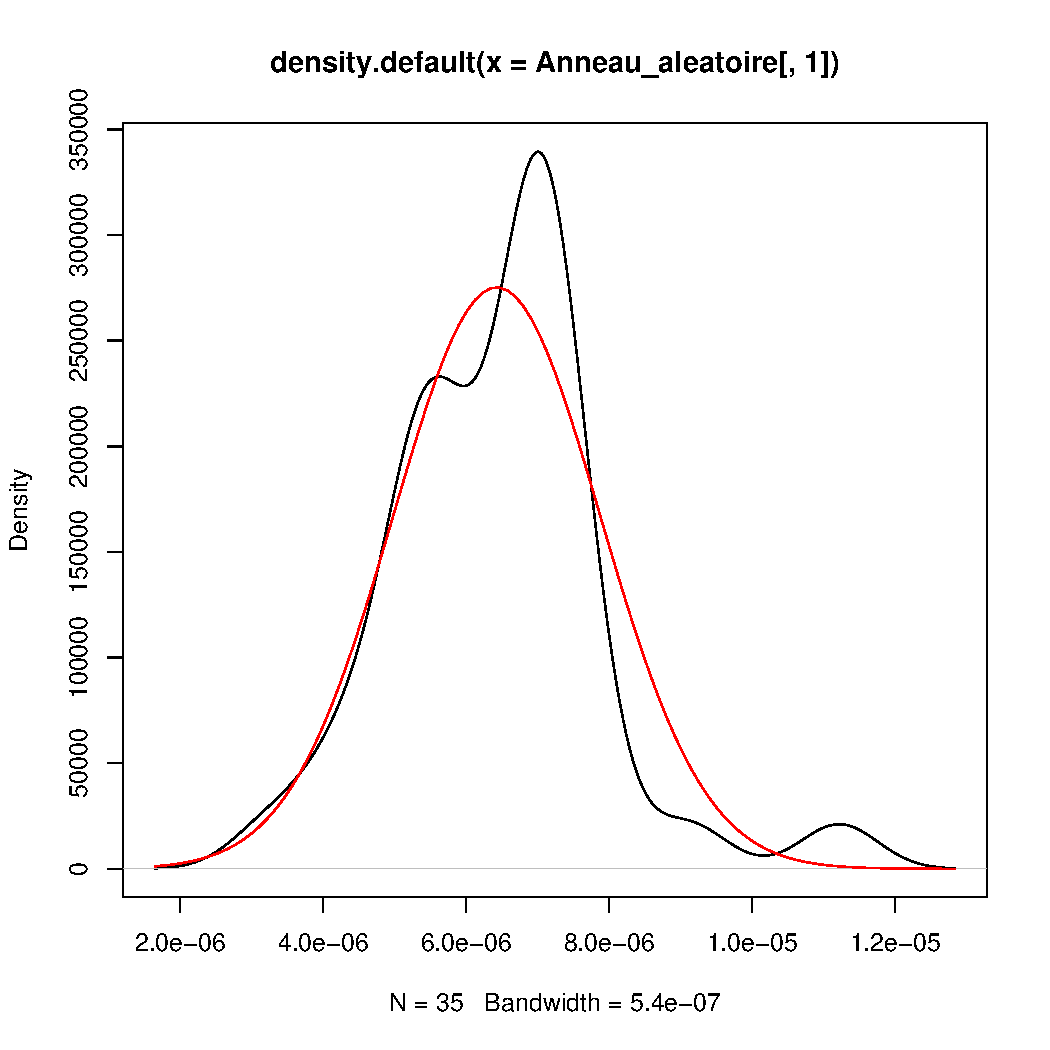
\includepdf[pages = {1-4}]{../R/Cible_perti_faible_graphe_alea/hist_alea_anneau.pdf}
	\subsection{Analyses Graphes complet}
	\subsection{Analyses Arbres}
	\subsection{Conclusion sur l'impact de chaque structure}
	\subsection{Conclusion sur l'impact en fonction de la pertinence de la cible}

\section{Conclusion}

\end{document}
